\section{Introduction to Embedded Linux}

\begin{frame}{Simplified Linux system architecture}
  \begin{center}
    \includegraphics[height=0.8\textheight]{slides/buildroot-introduction/linux-system-architecture.pdf}
  \end{center}
\end{frame}

\begin{frame}{Overall Linux boot sequence}
  \begin{center}
    \includegraphics[height=0.8\textheight]{slides/buildroot-introduction/overall-boot-sequence.pdf}
  \end{center}
\end{frame}

\begin{frame}{Embedded Linux work}
  \begin{itemize}
  \item {\bf BSP work}: porting the bootloader and Linux kernel,
    developing Linux device drivers.
  \item {\bf system integration work}: assembling all the userspace
    components needed for the system, configure them, develop the
    upgrade and recovery mechanisms, etc.
  \item {\bf application development}: write the company-specific
    applications and libraries.
  \end{itemize}
\end{frame}

\begin{frame}{Complexity of userspace integration}
  \begin{center}
    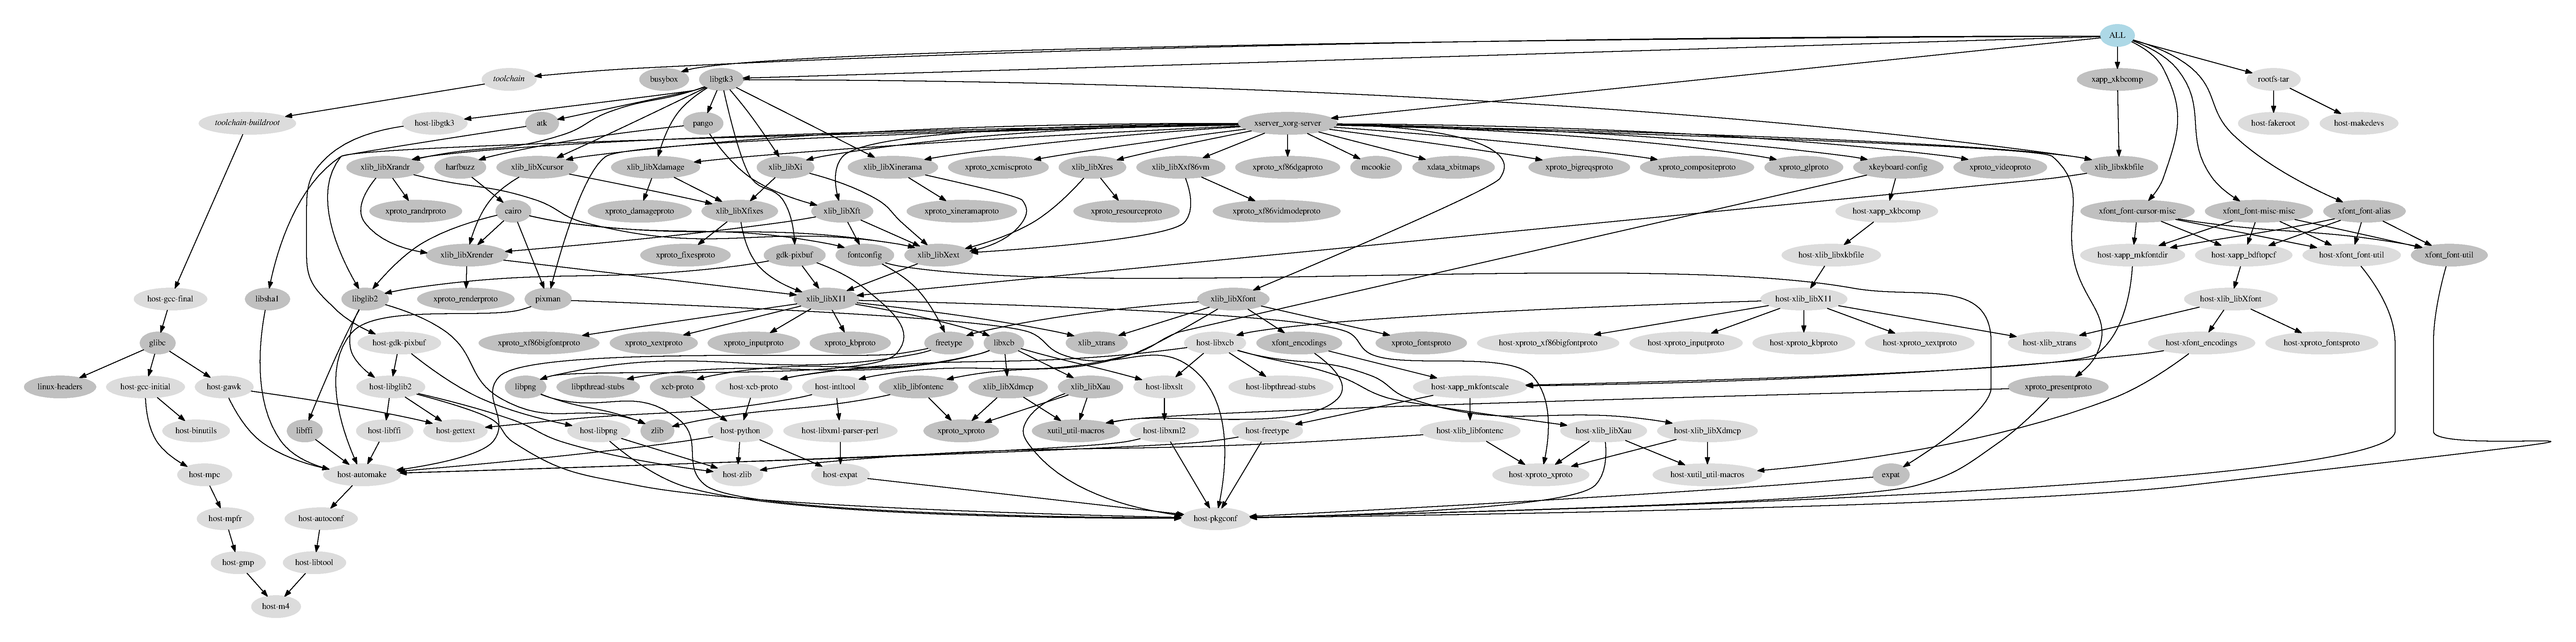
\includegraphics[width=\textwidth]{slides/buildroot-introduction/graph-depends.pdf}
  \end{center}
\end{frame}

\begin{frame}{System integration: several possibilities}
  \tiny
  \begin{tabularx}{11cm}{|X|X|X|}
    \hline
    & {\bf Pros} & {\bf Cons} \\
    \hline
    {\bf Building everything manually} &
    Full flexibility \newline
    Learning experience &
    Dependency hell \newline
    Need to understand a lot of details \newline
    Version compatibility \newline
    Lack of reproducibility \\
    \hline
    {\bf Binary distribution} \newline Debian, Ubuntu, Fedora, etc.
    &
    Easy to create and extend
    &
    Hard to customize \newline
    Hard to optimize (boot time, size) \newline
    Hard to rebuild the full system from source \newline
    Large system \newline
    Uses native compilation (slow) \newline
    No well-define mechanism to generate an image \newline
    Lots of mandatory dependencies \newline
    Not available for all architectures \\
    \hline
    {\bf Build systems} \newline Buildroot, Yocto, PTXdist, etc.
    &
    Nearly full flexibility \newline
    Built from source: customization and optimization are easy \newline
    Fully reproducible \newline
    Uses cross-compilation \newline
    Have embedded specific packages not necessarily in desktop distros \newline
    Make more features optional
    &
    Not as easy as a binary distribution \newline
    Build time \\
    \hline
  \end{tabularx}
\end{frame}

\begin{frame}{Embedded Linux build system: principle}
  \begin{center}
    \includegraphics[width=0.9\textwidth]{slides/buildroot-introduction/buildsystem-principle.pdf}
  \end{center}
  \begin{itemize}
  \item Building from source $\rightarrow$ lot of flexibility
  \item Cross-compilation $\rightarrow$ leveraging fast build machines
  \item Recipes for building components $\rightarrow$ easy
  \end{itemize}
\end{frame}

\begin{frame}{Embedded Linux build system: tools}
  \begin{itemize}
  \item A wide range of solutions: Yocto/OpenEmbedded, PTXdist,
    Buildroot, LTIB, OpenBricks, OpenWRT, and more.
  \item Today, two solutions are emerging as the most popular ones
    \begin{itemize}
    \item {\bf Yocto/OpenEmbedded}\\Builds a complete Linux
      distribution with binary packages. Powerful, but somewhat
      complex, and quite steep learning curve.
    \item {\bf Buildroot}\\Builds a root filesystem image, no binary
      packages. Much simpler to use, understand and modify.
    \end{itemize}
  \end{itemize}
\end{frame}

\section{Introduction to Buildroot}

\begin{frame}{Buildroot at a glance}
  \begin{itemize}
  \item Can build a toolchain, a rootfs, a kernel, a bootloader
  \item {\bf Easy to configure}: menuconfig, xconfig, etc.
  \item {\bf Fast}: builds a simple root filesystem in a few minutes
  \item Easy to understand: written in make, extensive documentation
  \item {\bf Small} root filesystem, starting at 2 MB
  \item {\bf 1600+ packages} for userspace libraries/apps available
  \item {\bf Many architectures} supported
  \item {\bf Well-known technologies} : {\em make} and {\em kconfig}
  \item Vendor neutral
  \item Active community, regular releases
    \begin{itemize}
    \item The present slides cover {\em Buildroot 2015.02}. There may
      be some differences if you use older or newer Buildroot version.
    \end{itemize}
  \item \url{http://buildroot.org}
  \end{itemize}
\end{frame}

\begin{frame}{Buildroot design goals}
  \begin{itemize}
  \item Buildroot is designed with a few key goals:
    \begin{itemize}
    \item Simple to use
    \item Simple to customize
    \item Reproducible builds
    \item Small root filesystem
    \item Relatively fast boot
    \item Easy to understand
    \end{itemize}
  \item Some of these goals require to not necessarily support all
    possible features
  \item They are some more complicated and featureful build systems
    available (Yocto Project, OpenEmbedded)
  \end{itemize}
\end{frame}

\begin{frame}{Who's using Buildroot?}
  \begin{columns}
    \column{0.6\textwidth}
    \begin{itemize}
    \item {\bf System makers}
      \begin{itemize}
      \item Google
      \item Barco
      \item Rockwell Collins
      \end{itemize}
    \item {\bf Processor vendors}
      \begin{itemize}
      \item Imagination Technologies
      \item Marvell
      \item Atmel
      \item Analog Devices
      \end{itemize}
    \item Many companies when doing {\em R\&D} on products
    \item Many, many {\bf hobbyists} on development boards:
      Rasberry Pi, BeagleBone Black, etc.
  \end{itemize}
  \column{0.4\textwidth}
  \only{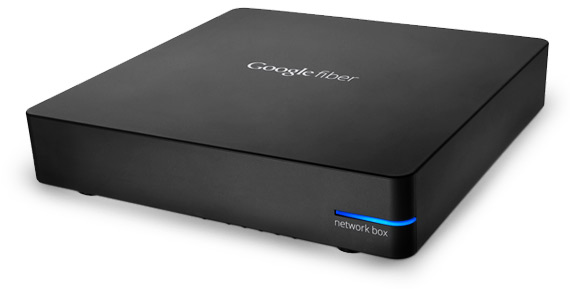
\includegraphics[width=0.8\textwidth]{slides/buildroot-introduction/google-fiber-box.jpg}}\\
  \only{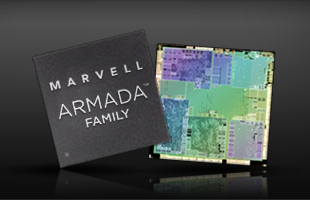
\includegraphics[width=0.8\textwidth]{slides/buildroot-introduction/armada.jpg}}\\
  \only{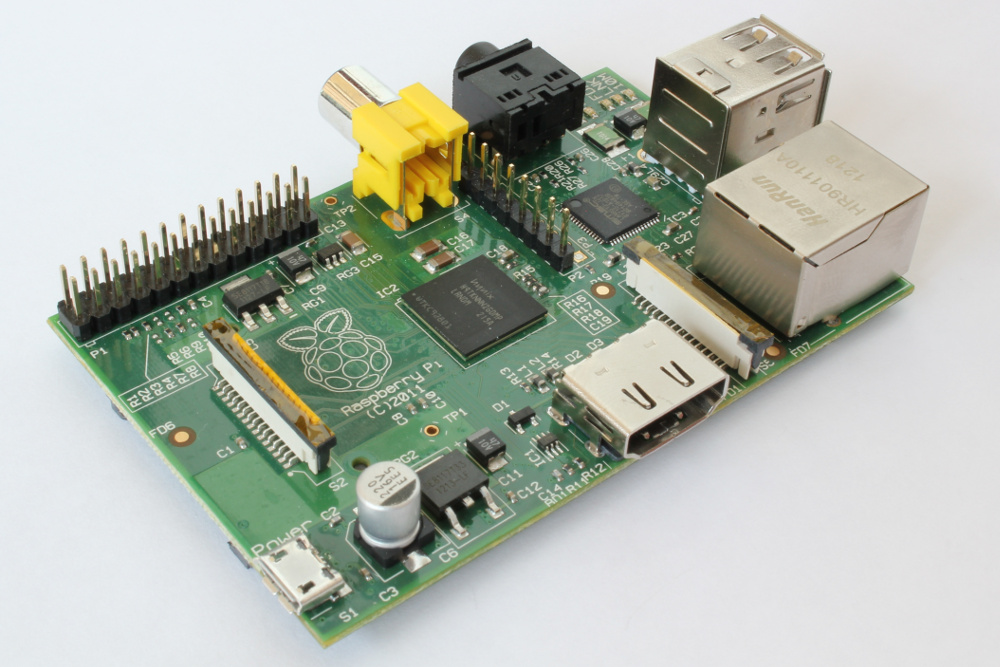
\includegraphics[width=0.8\textwidth]{slides/buildroot-introduction/rasberrypi.jpg}}
  \end{columns}
\end{frame}

\begin{frame}{Getting Buildroot}
  \begin{itemize}
  \item Stable Buildroot releases are published every three months.
  \item Tarballs are available for each stable release
    \begin{itemize}
    \item \url{http://buildroot.org/downloads/}
    \end{itemize}
  \item However, it is generally more convenient to clone the Git
    repository
    \begin{itemize}
    \item Allows to clearly identify the changes you make to the
      Buildroot source code
    \item Simplifies the upstreaming of the Buildroot changes
    \item \code{git clone git://git.busybox.net/buildroot}
    \item Git tags available for every stable release.
    \end{itemize}
  \end{itemize}
\end{frame}

\begin{frame}[fragile]{Using Buildroot}
  \begin{itemize}
  \item Implemented in \code{make}
    \begin{itemize}
    \item With a few helper shell scripts
    \end{itemize}
  \item All interaction happens by calling \code{make} in the main Buildroot
    sources directory.
    \begin{block}{}
\begin{verbatim}
$ cd buildroot/
$ make help
\end{verbatim}
    \end{block}
  \item No need to run as \code{root}, Buildroot is designed to be
    executed with normal user privileges.
    \begin{itemize}
    \item Running as root is even strongly discouraged!
    \end{itemize}
  \end{itemize}
\end{frame}

\begin{frame}{Configuring Buildroot}
  \begin{itemize}
  \item Like the Linux kernel, uses {\em Kconfig}
  \item A choice of configuration interfaces:
    \begin{itemize}
    \item \code{make menuconfig}
    \item \code{make nconfig}
    \item \code{make xconfig}
    \item \code{make gconfig}
    \end{itemize}
  \item Make sure to install the relevant libraries in your system
    ({\em ncurses} for menuconfig/nconfig, {\em Qt} for xconfig, {\em
      Gtk} for gconfig)
  \end{itemize}
\end{frame}

\begin{frame}{Main {\tt menuconfig} menu}
  \begin{center}
    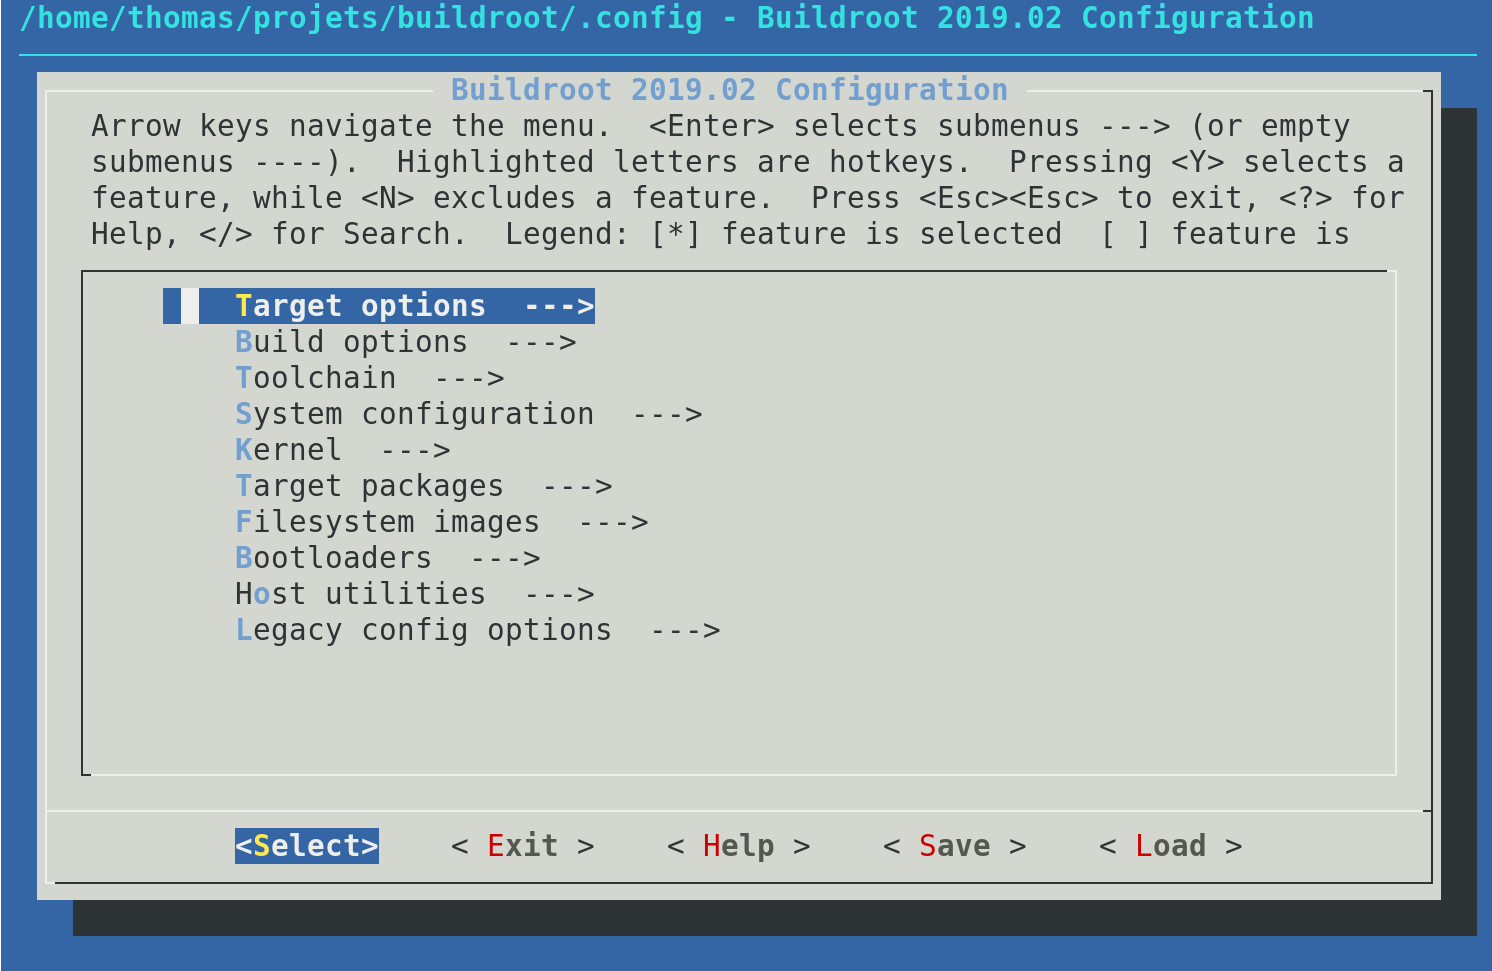
\includegraphics[width=\textwidth]{slides/buildroot-introduction/menuconfig.png}
  \end{center}
\end{frame}

\begin{frame}[fragile]{Running the build}
  \begin{itemize}
  \item As simple as:
    \begin{block}{}
\begin{verbatim}
$ make
\end{verbatim}
    \end{block}
  \item Often useful to keep a log of the build output, for analysis
    or investigation:
    \begin{block}{}
\begin{verbatim}
$ make 2>&1 | tee build.log
\end{verbatim}
    \end{block}
  \end{itemize}
\end{frame}

\begin{frame}{Build results}
  \begin{itemize}
  \item The build results are located in \code{output/images}
  \item Depending on the configuration, this directory will contain:
    \begin{itemize}
    \item One or several root filesystem images, in various formats
    \item One kernel image, possibly one or several Device Tree blobs
    \item One or several bootloader images
    \end{itemize}
  \item There is no standard way to install the images on any given
    device
    \begin{itemize}
    \item Those steps are very device specific
    \item Buildroot provides some tools for specific platforms (e.g.:
      SAM-BA for Atmel, imx-usb-loader for i.MX6, etc.)
    \end{itemize}
  \end{itemize}
\end{frame}

\setuplabframe
{Basic Buildroot usage}
{
  \begin{itemize}
  \item Get Buildroot
  \item Configure a minimal system with Buildroot for the BeagleBone
    Black
  \item Do the build
  \item Prepare the BeagleBone Black for usage
  \item Flash and test the generated system
  \end{itemize}
}
